\begin{figure*}[t]
    \centering
    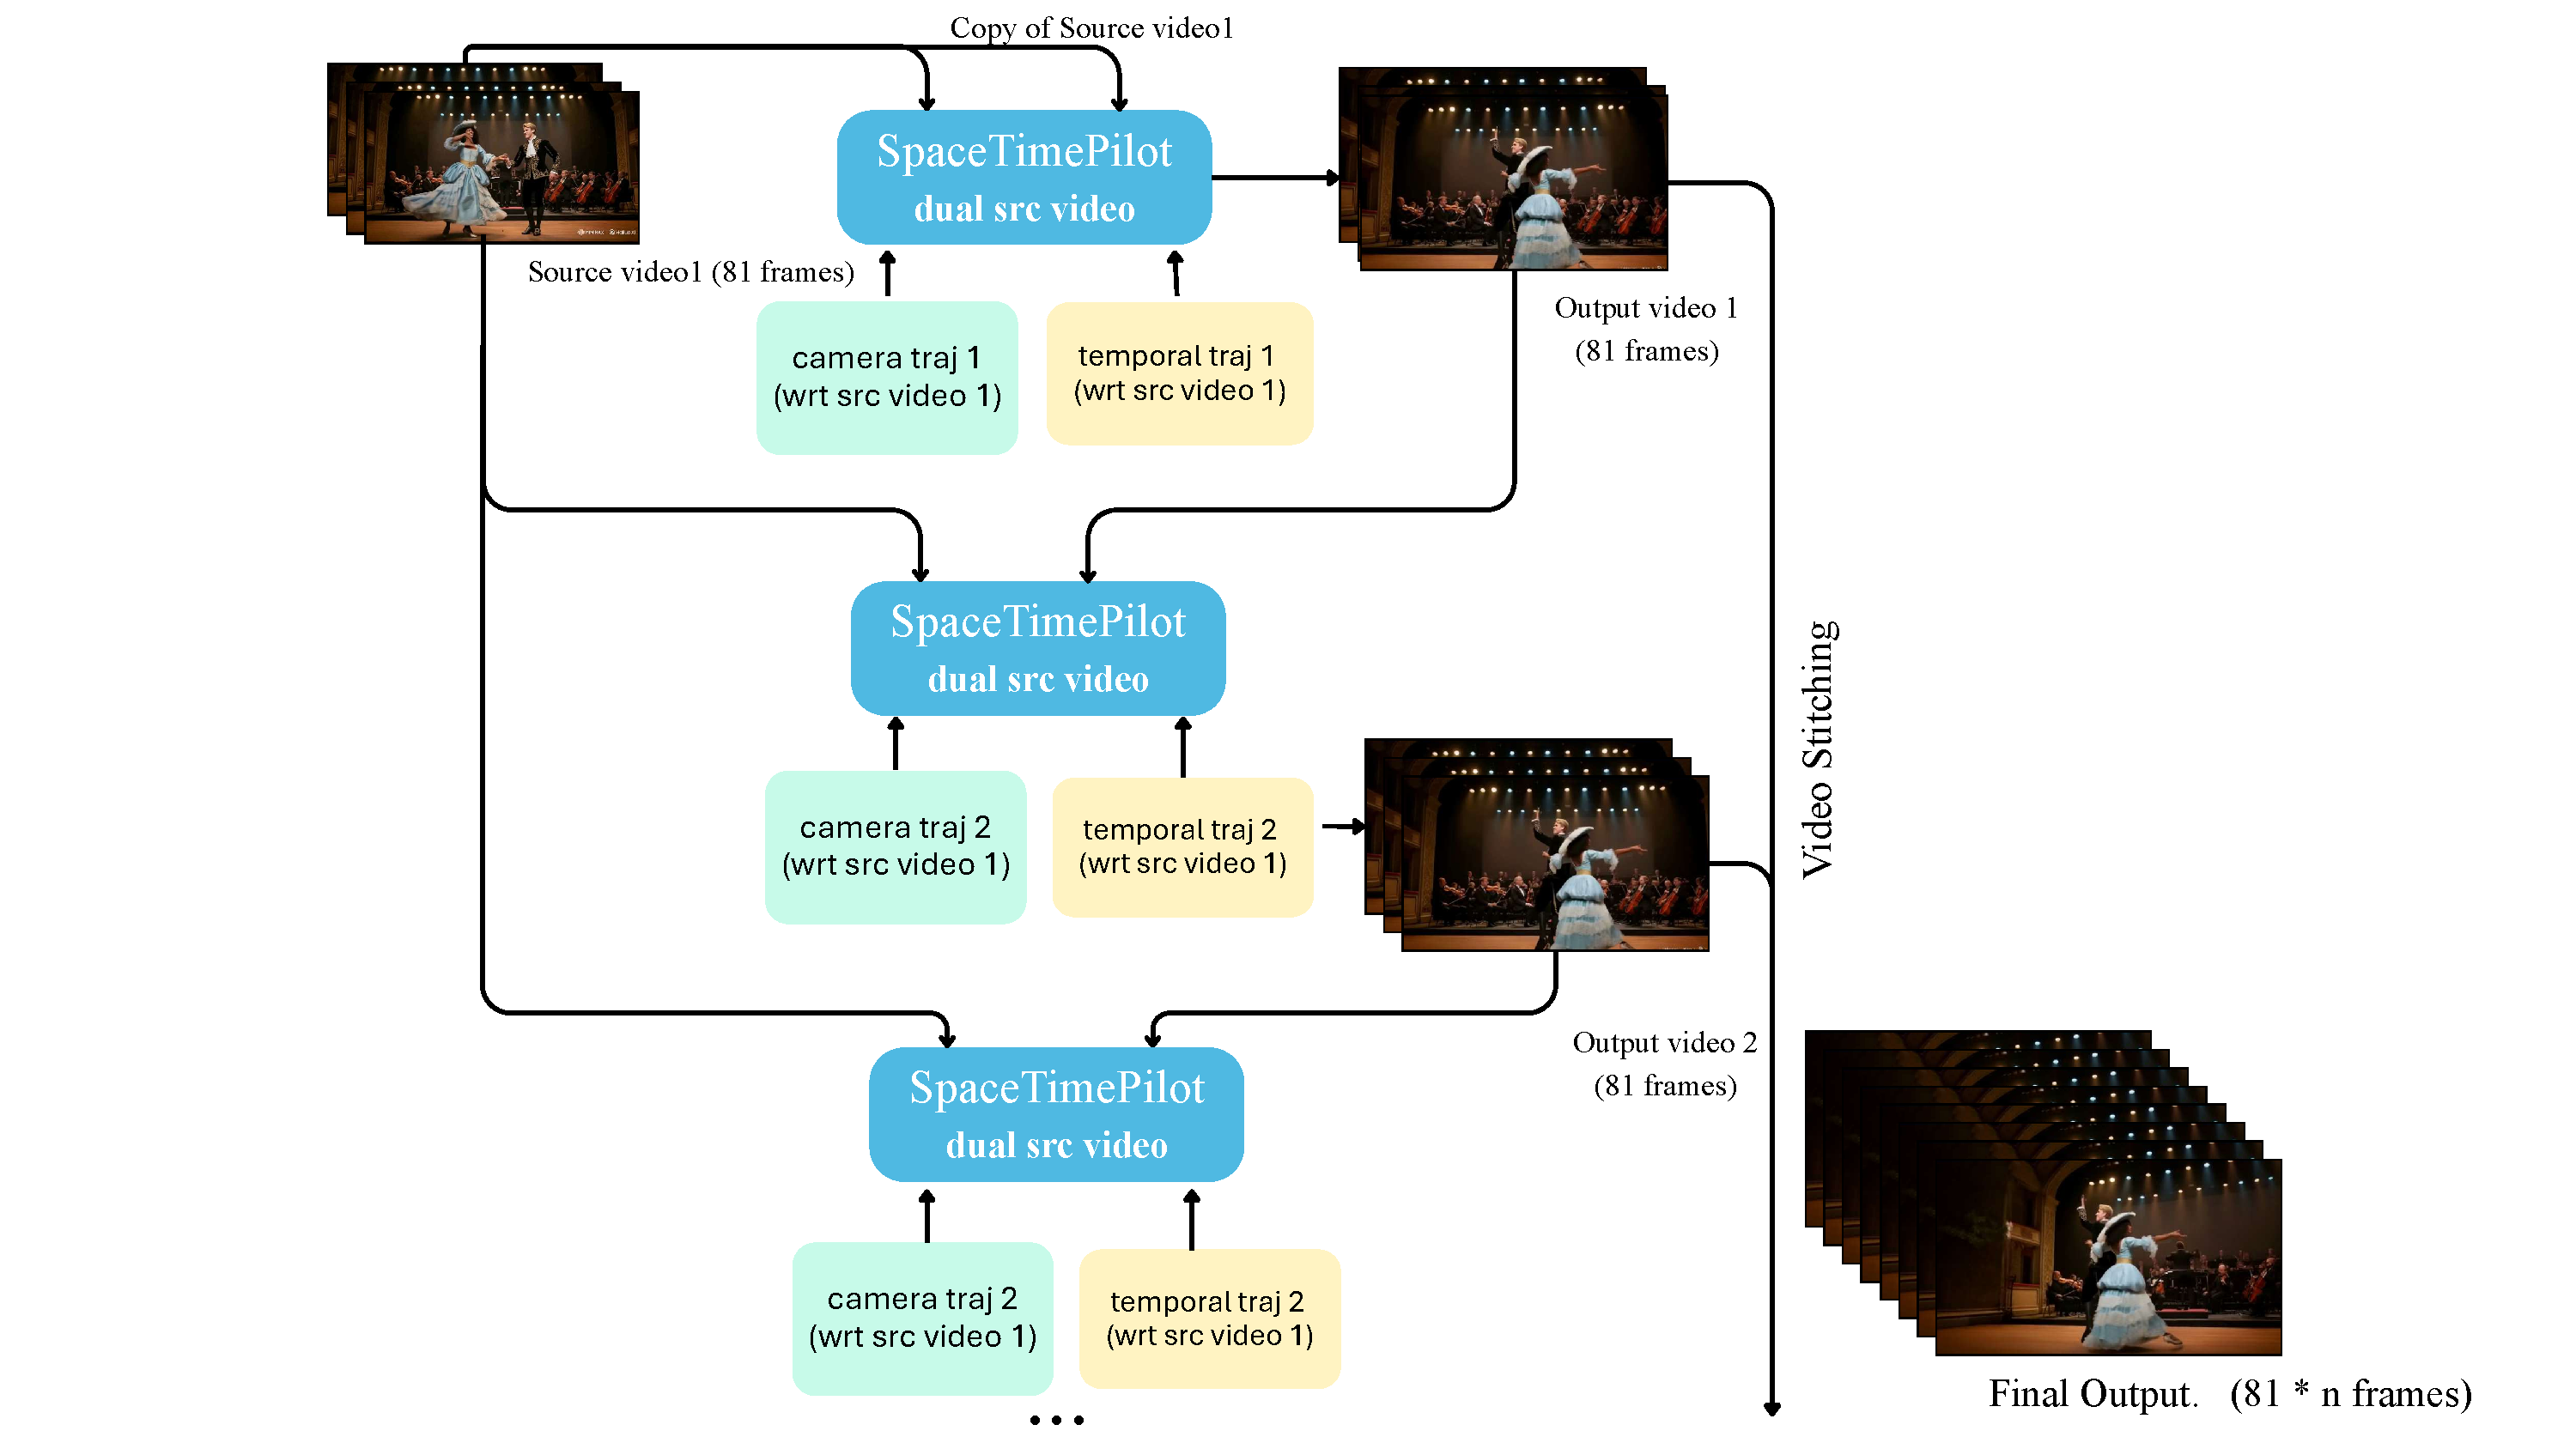
\includegraphics[width=\linewidth]{figures/AR-pipeline.pdf}
    \caption{
        \textbf{Overview of the multi-turn autoregressive inference scheme.}
The model first generates an 81-frame segment conditioned on the source video and a chosen space–time trajectory. The resulting output is then reused as a secondary source video for subsequent iterations, each with its own camera and temporal trajectory. By chaining these iterations and stitching the outputs, \nameMethod produces a long, coherent video that follows an arbitrary space–time path.
    }
    \label{fig:multi-turn}
\end{figure*}

\section{Longer Space-Time Exploration Video with Disentangled Controls}

 One of the central advantages of \nameMethod is its ability to freely navigate both spatial and temporal dimensions, with arbitrary starting points in each dimension and fully customizable trajectories through them. Although each individual generation is limited to an 81-frame window, we show that \nameMethod can effectively extend this window indefinitely through a multi-turn autoregressive inference scheme, enabling continuous and controllable space–time exploration from a single input video. The overall pipeline is illustrated in \cref{fig:multi-turn}.

The core idea is to generate the final video in autoregressive segments that connect seamlessly.  For example, given a source video of 81 frames, we may first generate a 0.5$\times$ slow-motion sequence covering frames 0–40 with a new camera trajectory. Then, continuing both the visual context and the generated camera trajectory, we can produce the next segment starting from the final camera pose of the previous output, while temporally traversing the remaining frames 40–81. This yields an autoregressive chain of viewpoint-controlled video segments that together create a continuous long-range space–time trajectory.

A key property that enables this behavior is that our model can generate video segments whose camera poses do \emph{not} need to start at the first frame. 
This allows precise control over the starting point, both in time and viewpoint, for every generated chunk, ensuring smooth, consistent motion over extended sequences.

To maintain contextual coherence across iterations, we introduce a lightweight memory mechanism. During training, the model is conditioned on \textbf{a pair of source videos}, which enables consistent chaining during inference. Specifically:
\begin{itemize}
\item At iteration $i = 1$, the model is conditioned only on the original source video.
\item At iteration $i = 2$, it is conditioned on both the source video and the previously generated 81-frame segment.
\item This process repeats, with each iteration conditioning on the source video as well as the most recent generated segment.
\end{itemize}

This simple yet effective strategy allows \nameMethod to generate arbitrarily long, smoothly connected sequences with continuous and precise control over both temporal manipulation and camera motion.

Here, we showcase how this can be used to conduct large viewpoint changes, as demonstrated in \cref{fig:multi-turn demo}.



\begin{figure*}[t]
    \vspace{-5mm}
    \centering
    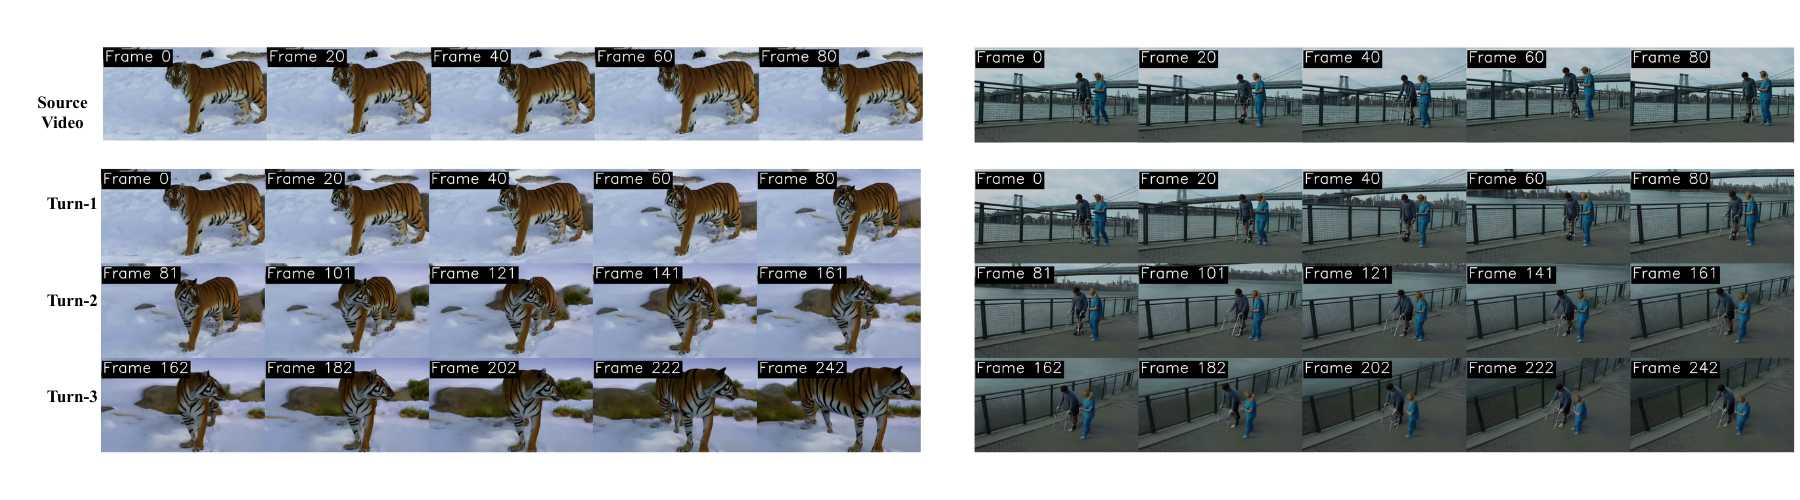
\includegraphics[width=\linewidth]{figures/src_files/ar_demo.jpg}
    \vspace{-1Cm}
    \caption{
       \textbf{ Multi-turn autoregressive generation with \nameMethod.} Top row: source video frames.
Rows 2–4: Turn-1, Turn-2, and Turn-3 generations.
At each turn, \nameMethod jointly conditions on (1) the original source video and (2) the previously generated chunk, ensuring temporal continuity, stable motion progression, and consistent camera geometry.
This dual-conditioning design enables viewpoint changes far beyond the input video—such as rotating to the rear of the tiger or transitioning from a low-angle shot to a high bird’s-eye view—while preserving visual and motion coherence. Please refer to section ``AR Demos'' in the website for videos.
    }
    \label{fig:multi-turn demo}
\end{figure*}


